
\section*{\documentclass{article}
\usepackage{graphicx} % Required for inserting images
\usepackage{caption} % Required for \captionof
\usepackage{amsmath}
\usepackage{float}
\usepackage{comment}
\usepackage[T1]{fontenc}
\usepackage[utf8]{inputenc}
\usepackage{lmodern}
\usepackage{microtype}
\usepackage{xcolor}
\usepackage{framed}
\renewenvironment{leftbar}{%
  \def\FrameCommand{\textcolor{orange}{\vrule width 3pt} \hspace{10pt}}%
  \MakeFramed {\advance\hsize-\width \FrameRestore}}%
 {\endMakeFramed}

\title{Mechanikai mérés}
\author{Kern Luca, Vincze Csongor}
\date{2026 Április 22}

\begin{document}

\maketitle

\section*{4. Feladat: Igazolja a Steiner-tételt!}

Steiner-tétel: $\theta' = \theta + mr^2.$

$m_{piros csap}= 2,08 \text{kg}$

$r_{korong-középpont}= \text{m}$
$T_{lengési}= \text{s}$

Első mérési pont:
1. mérés: $r_{korong-középpont}= \text{m}$,$T_{lengési}= \text{s}$

\begin{figure}[H]
    \centering
    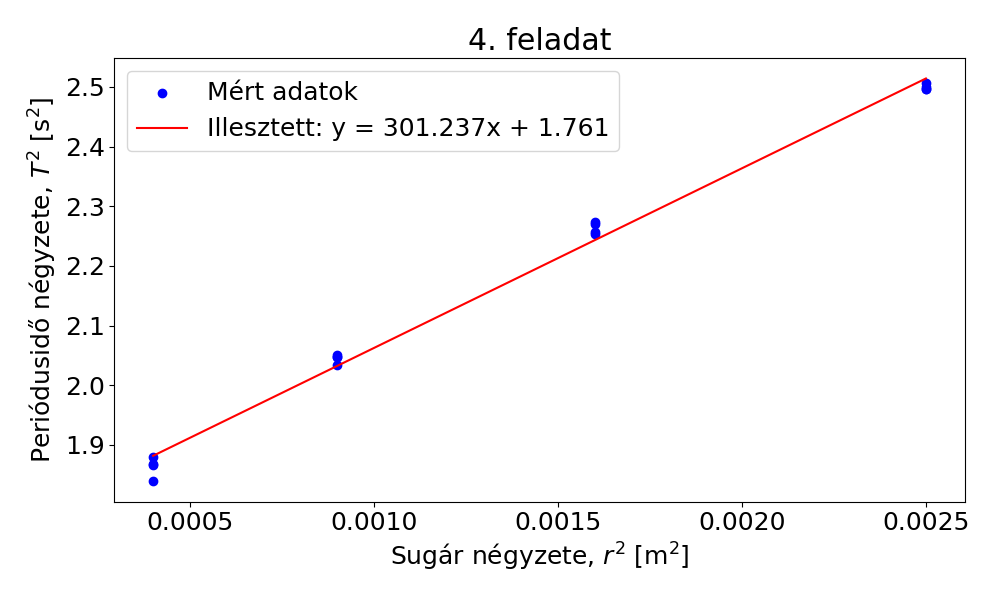
\includegraphics[width=0.8\textwidth]{4_feladat.png}
    \caption{Szögkitérés mértékének függése a golyók számától}
    \label{fig:4}
\end{figure}

A direkcoós állandóra 6,74*10^-3 Nm adódott

\end{document}
